\chapter{مقایسه\nf کیفیت سرویس در \lr{IMS} و \lr{VOIP}}
\setlatintextfont{Times New Roman}
\section{نیاز به کیفیّت سرویس}

همانطور که در فصل \ref{fasleavval} توضیح داده\nf شد، مزیت اصلی \lr{IMS} نسبت به سیستم\nf های متداول \lr{VOIP}، تضمین کیفیّت سرویس در مکالمات است. شبکه\nf ی اینترنت و پروتکل\nf های استفاده\nf شده در این شبکه، هیچگونه تضمینی برای برقراری سطح خاصی از کیفیّت سرویس را ارائه نمی\nf کنند\RTLfootnote{شبکه\nf های \lr{ATM} می\nf توانند با اختصاص لینک اختصاصی به هر ارتباط، کیفیّت سرویس مورد نیاز را ارائه دهند}}. از طرفی، اپلیکیشن\nf های مختلف، نیار دارند که پروتکل\nf های لایه\nf ی انتقال، حدّاقل\nf های مورد نیازشان را تأمین کند. 


این نیازها که به سه بخش تقسیم می\nf شوند،عبارتند از: نیاز به قابل اعتماد بودن و عدم از دست رفتن داده\nf ها، نیاز به حداقل نرخ ارسال(دریافت) داده\nf ها\RTLfootnote{\lr{Throughput}} و حساسیّت نسبت به زمان. اپلیکیشن\nf هایی که برای تماس صوتی و یا ویدیوئی مورد استفاده قرار می\nf گیرند، نسبت به از دست رفتن داده\nf ها، حسّاسیت کمی دارند و می\nf توانند با وجود از دست رفتن بخشی از داده\nf ها، سرویس موردنظر را به\nf درستی ارائه کنند. امّا این اپلیکیشن\nf ها، شدیداً وابسته به نرخ ارسال(دریافت) هستند و حسّاسیات بالایی نیز نسبت به زمان دارند؛ به\nf طوری که در صورت کم بودن نرخ ارسال(دریافت) داده\nf ها و زیاد بودن زمان رفت و برگشت\RTLfootnote{\lr{Round Trip Time(RTT)}}، قادر به ارائه\nf ی سرویس نیستند. همچنین، باتوجّه به شرایط فوق، امکان دارد کیفیت سرویس ارائه\nf شده پایین بیاید و باعث نارضایتی کاربر شود\cite{cn}.

\section{مقایسه\nf ی کیفیت سرویس در شبکه اینترنت}

سیستم\nf های مبتنی بر پروتکل \lr{SIP}، به صورت مستقیم در تبادل مدیا شرکت نمی\nf کنند و فقط سیگنالینگ\nf های لازم برای برقراری، کنترل و خاتمه\nf ی ارتباط را انجام می\nf دهند. در واقع می\nf توان گفت که اپلیکیشن\nf های مبتنی بر پروتکل \lr{SIP}، وظیفه\nf ی ایجاد و کنترل یک ارتباط نظیر به نظیر\RTLfootnote{\lr{peer to peer}} بین تماس\nf گیرنده و مخاطب وی را برعهده دارند\cite{blended}. کیفیّت سرویس ارائه\nf شده نیز بیشتر مربوط به مدیا می\nf باشد و سیگنال\nf های مبادله\nf شده، تأثیر چندانی در میزان کیفیّت سرویسی که کاربر تجربه می\nf کند، ندارند. لذا، می\nf توان گفت که کیفیّت سرویس، در صورت استفاده از \lr{IMS} به عنوان یک سرویس \lr{VOIP} در شبکه\nf ی اینترنت و یا شبکه\nf های محلی، تفاوت چندانی با استفاده از سایر سیستم\nf های \lr{VOIP} ندارد. 

برای ایجاد کیفیت سرویس در مدیای مبادله\nf شده، می\nf توان از روش\nf هایی مانند \lr{MPLS}\RTLfootnote{سرواژه\nf ی عبارت \lr{Multi Protocol Label Switching} و به معنای سوئیچینگ برچسب\nf های چندپروتکل} و یا \lr{Diffserv}\RTLfootnote{کوتاه\nf شده\nf ی عبارت \lr{Differentiated Service} و به معنای سرویس تفاوت قائل\nf شده می\nf باشد.} استفاده کرد. روش \lr{MPLS}، مشابه روش شبکه\nf های مدار مجازی عمل می\nf کند\RTLfootnote{\lr{virtual circuit network}}. البتّه، مسیریاب\nf های موجود در مسیر طرفین مکالمه، باید همگی از \lr{MPLS} پشتیبانی کنند. روش \lr{Diifserve} نیز از طریق تفاوت قائل شدن بین سرویس\nf های مختلف و در نظرگرفتن اولویّت بالاتر برای عبور بسته\nf های سرویس\nf های مکالمه\nf ای، باعث بالا رفتن نرخ ارسال و کاهش زمان ارسال این نوع بسته\nf ها می\nf شود\cite{cn}.


استفاده از روش \lr{MPLS} و \lr{Diffserv}، مربوط به پیکربندی شبکه\nf ی محلّی و یا شبکه\nf ی اینترنت می\nf باشد. لذا ممکن است که شبکه\nf ی موردنظر، استفاده از این دو روش را پشتیبانی نکند. همچنین، سیستم\nf های \lr{VOIP} متداول نیز می\nf توانند مانند \lr{IMS}، از این روش\nf ها بهره\nf مند شوند. \lr{IMS} نیز مانند برخی سیستم\nf های \lr{VOIP} نظیر \lr{Asterisk}، پروتکل \lr{SIP} را با استفاده از \lr{pjsip} پیاده\nf سازی کرده\nf است. \lr{pjsip}، یک پشته\nf ی پروتکل ِ\RTLfootnote{\lr{Protocol Stack}} \lr{SIP} است که با زبان برنامه\nf نویسی \lr{C} نوشته\nf شده و متن\nf باز است. \lr{pjsip}، قابلیت استفاده از \lr{Diffserv} و قرار دادن مقدار مربوط به اولویّت در سرآمد بسته\nf های \lr{IP} و همچنین برخی روش\nf های دیگر برای ایجاد کیفیّت سرویس را دارد\cite{webpjsip}.


با توجّه به مطالب گفته\nf شده و از آنجایی\nf که \lr{pjsip}، توسّط سایر سیستم\nf های \lr{VOIP} نیز استفاده می\nf شود، می\nf توان نتیجه گرفت که در بخش مدیای مبادله\nf شده(در صورت استفاده ز \lr{IMS} به\nf عنوان سرور \lr{VOIP} در بستر اینترنت)، تفاوتی بین \lr{IMS} و سایر سیستم\nf های \lr{VOIP} وجود ندارد. بنابراین، استفاده از شبیه\nf سازی برای مقایسه\nf ی کیفیّت سرویس در مدیای مبادله\nf شده توسّط کاربران این سیستم\nf ها، کاری بیهوده است. لذا، سیگنالینگ\nf های مورد استفاده در این دو سیستم مورد بررسی قرار می\nf گیرند تا مشخّص شود که آیا سیستم \lr{IMS} به عنوان یک ارائه\nf دهنده\nf ی \lr{VOIP}، نسبت به سایر سیستم\nf های متداول \lr{VOIP} برتری دارد یا خیر.


\subsection{مقایسه\nf ی سیگنالینگ \lr{VOIP} و \lr{IMS} در شبکه\nf ی اینترنت}
\subsubsection{بستر ایجادشده برای انجام مقایسه}
در این بخش، سیگنالینگ\nf های مربوط به ثبت\nf نام و برقراری تماس \lr{VOIP} و \lr{IMS}(به\nf عنوان ارائه\nf دهنده\nf ی سرویس \lr{VOIP}) مورد بررسی قرار می\nf گیرند. سیستم\nf های \lr{IMS} و \lr{VOIP}، هر دو به\nf صورت ماشین مجازی بر روی سکّوی مجازی\nf سازی \lr{Virtualbox} نصب شدند. پیاده\nf سازی \lr{IMS}، به\nf صورت سیستم یکپارچه بر روی سکّوی مجازی\nf سازی انجام شد(بخش \ref{cwaio}). نسخه\nf ی \lr{13} نرم\nf افزار \lr{Asterisk}\cite{asterisk} نیز به\nf عنوان سرور \lr{VOIP} بر روی ماشین مجازی لینوکس اوبونتو \lr{16.04} نصب شد. اپلیکیشن \lr{zoiper} نیز به\nf عنوان اپلیکشن سمت کاربر مورد استفاده قرار گرفت. 

اپلیکشن \lr{zoiper}، از طریق ارسال پیام\nf های سیگنالینگ به سیستم میزبان(سیستمی که سکّوی مجازی\nf سازی بر روی آن نصب شده است)، عمل ثبت\nf نام کاربر در سیستم را انجام می\nf دهد. سیستم میزبان و دستگاه کاربر، با اتّصال به مودم وای\nf فای، آدرس \lr{IP} خود را به\nf دست می\nf آورند. برای ارتباط با \lr{clearwater}، لازم است که اپلیکیشن کاربر، به آدرس \lr{IP} سیستم میزبان دسترسی داشته باشد و پیام\nf ها، به\nf طور مستقیم به ماشین مجازی موردنظر فرستاده نمی\nf شوند؛ بلکه پیام\nf ها از طریق ماشین میزبان، به ماشین مجازی \lr{clearwater}(از طریق آداپتور شبکه\nf ی \lr{NAT}) فرستاده می\nf شوند. برای ارتباط با سرور \lr{Asterisk}، اپلیکیشن کاربر باید پیام\nf های \lr{SIP} را مستقیماً به ماشین مجازی که \lr{Asterisk} بر روی آن نصب شده است، بفرستد. لذا آداپتور شبکه\nf ی این ماشین مجازی، در حالت \lr{Bridge} قرار داده\nf شد.

مودم وای\nf فای، به ماشین میزبان، ماشین مجازی لینوکس(سرور \lr{Asterisk}) و دستگاه کاربر، به\nf ترتیب آدرس \lr{IP} های \lr{192.168.1.106}، \lr{192.168.1.107} و \lr{192.168.1.104} را اختصاص داد. \lr{zoiper}، پیام\nf های سیگنالینگ برای ارتباط با \lr{IMS} را به آدرس \lr{IP} سیستم میزبان می\nf فرستد. همچنین، پیام\nf های سیگنالینگ برای ارتباط با \lr{Asterisk} نیز به آدرس \lr{IP} ماشین مجازی لینوکس فرستاده میشوند. این دو آدرس \lr{IP}، هر دو مربوط به اینترفیس وای\nf فای سیستم میزبان می\nf باشند. لذا با \lr{capture} کردن بسته\nf های عبوری از اینترفیس وای\nf فای سیستم میزبان توسّط نرم\nf افزار وایرشارک، می\nf توان پیام\nf های \lr{SIP} مبادله\nf شده بین دستگاه کاربر و سرور \lr{IMS} و سرور \lr{Asterisk} را مشاهده کرد. 

\subsubsection{ثبت\nf نام  \lr{SIP}}

پس از پیکربندی \lr{zoiper} برای اتّصال به سرور \lr{IMS} و سرور \lr{VOIP}، عمل ثبت\nf نام به\nf طور خودکار توسّط این اپلیکیشن انجام می\nf شود. عمل ثبت\nf نام \lr{SIP}، در چهار مرحله انجام می\nf شود(شکل \ref{sipregister}). در مرحله\nf ی اوّل(\lr{F1})، کاربر درخواست ثبت\nf نام \lr{SIP} را به سرور \lr{SIP} ارسال می\nf کند. این درخواست، شامل نام\nf کاربری(همان شماره\nf ی تلفن)، آدرس \lr{IP} و یا دامنه\nf ی کاربر، اپلیکیشن مورد استفاده توسّط کاربر و برخی اطّلاعات دیگر می\nf باشد. از آنجایی\nf که سرور نمی\nf تواند از طریق این اطّلاعات که به\nf صورت متن عادی ارسال شده\nf اند، احراز هویّت را انجام دهد\RTLfootnote{به\nf دلیل مسائلی که در زمینه\nf ی امنیّت شبکه وجود دارد، ارسال رمز عبور نمی\nf تواند احراز هویّت را به\nf درستی انجام دهد.}، این درخواست ثبت\nf نام مورد قبول واقع نمی\nf شود\cite{rfcsip}.


\begin{figure}[h]
\centering
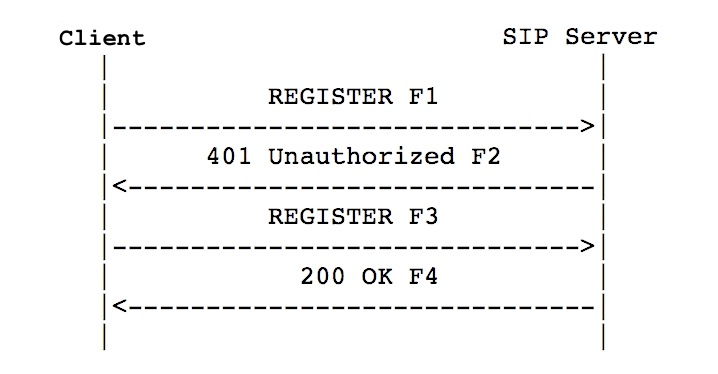
\includegraphics[width=0.7\textwidth]{sipregister}
\caption{ثبت\nf نام \lr{SIP}}
\label{sipregister}
\end{figure}

در مرحله\nf ی دوّم(\lr{F2})، سرور \lr{SIP}،  یک چالش امنیتی برای کاربر ایجاد می\nf کند تا بتواند از طریق آن، احراز هویّت را انجام بدهد. این احراز هویّت، برای ایجاد امنیّت و جلوگیری از حملاتی مانند حمله\nf ی مرد میانی\RTLfootnote{\lr{Man In The Middle Attack}} و حمله\nf ی بازپخش\RTLfootnote{\lr{Replay attack}} لازم است. کاربر با حل چالش مطرح\nf شده، می\nf تواند هویّت خود را برای سرور اثبات کند. در این چالش، سرور \lr{SIP} اطّلاعاتی نظیر روش احراز هویّت، الگوریتم مورداستفاده و عدد یک\nf بار مصرف\RTLfootnote{\lr{Nonce}. یک عدد تصادفی که توسّط سرور ایجاد می\nf شود تا کاربر، در محاسبات الگوریتم احراز هویّت، این عدد را نیز دخالت بدهد. با این کار، از حمله\nf ی بازپخش جلوگیری می\nf شود.}را برای کاربر مشخّص می\nf کند\cite{rfcsip}. 


در مرحله\nf ی سوّم(\lr{F3})، کاربر باید با استفاده از رمزعبور خود، اطّلاعات دریافت\nf شده از سمت سرور را به\nf وسیله\nf ی الگوریتم موردنظر رمز کند و خروجی به\nf دست\nf آمده را به سرور ارسال کند. سرور نیز الگوریتم موردنظر را با همین ورودی\nf ها و رمزعبور\RTLfootnote{رمزعبور کاربر در سرور موجود است.} اجرا می\nf کند. در صورت برابر بودن خروجی این الگوریتم با مقداری که کاربر ارسال کرده است، احراز هویّت انجام می\nf شود و سرور، ثبت\nf نام  را تأیید می\nf کند. در مرحله\nf ی آخر(\lr{F4})، سرور به کاربر اطّلاع می\nf دهد که ثبت\nf نام، با موفقیّت انجام شد\cite{rfcsip}.


\subsubsection{مقایسه\nf ی بسته\nf های ارسالی و دریافتی}

در هر دو سرور(\lr{IMS} و \lr{Asterisk})، پیام\nf های مبادله\nf شده برای ثبت\nf نام \lr{SIP}، منطبق بر استانداردهای پروتکل \lr{SIP} است که در بخش قبل توضیح داده شد. پیکربندی این سیستم \lr{IMS} به\nf گونه\nf ای است که از پروتکل لایه\nf ی انتقال \lr{TCP}\RTLfootnote{به\nf راحتی می\nf توان این پیکربندی را طوری تغییر داد که از پروتکل \lr{UDP} استفاده کند.} استفاده می\nf کند(شکل \ref{imssip}) امّا سرور \lr{Asterisk} مورد استفاده، از پروتکل \lr{UDP}(شکل \ref{voipsip}) استفاده می\nf کند. لذا، باتوجّه به قابل اعتماد بودن پروتکل \lr{TCP}، علاوه بر پیام\nf های \lr{SIP} مبادله\nf شده، بسته\nf های ACK نیز ارسال می\nf شوند\cite{cn}. زمان بین اوّلین درخواست ثبت\nf نام توسّط کاربر و پایان ثبت\nf نام، هم در \lr{IMS} و هم در \lr{VOIP}، حدود چندهزارم ثانیه است. لذا، با توجّه به نوسانات موجود در شبکه و تفاوت بسیار اندک در مدّت\nf زمان ثبت\nf نام، نمی\nf توان در مورد سرعت سیستم\nf های موردنظر در انجام این کار اظهارنظر کرد.

\begin{figure}[h]
\centering
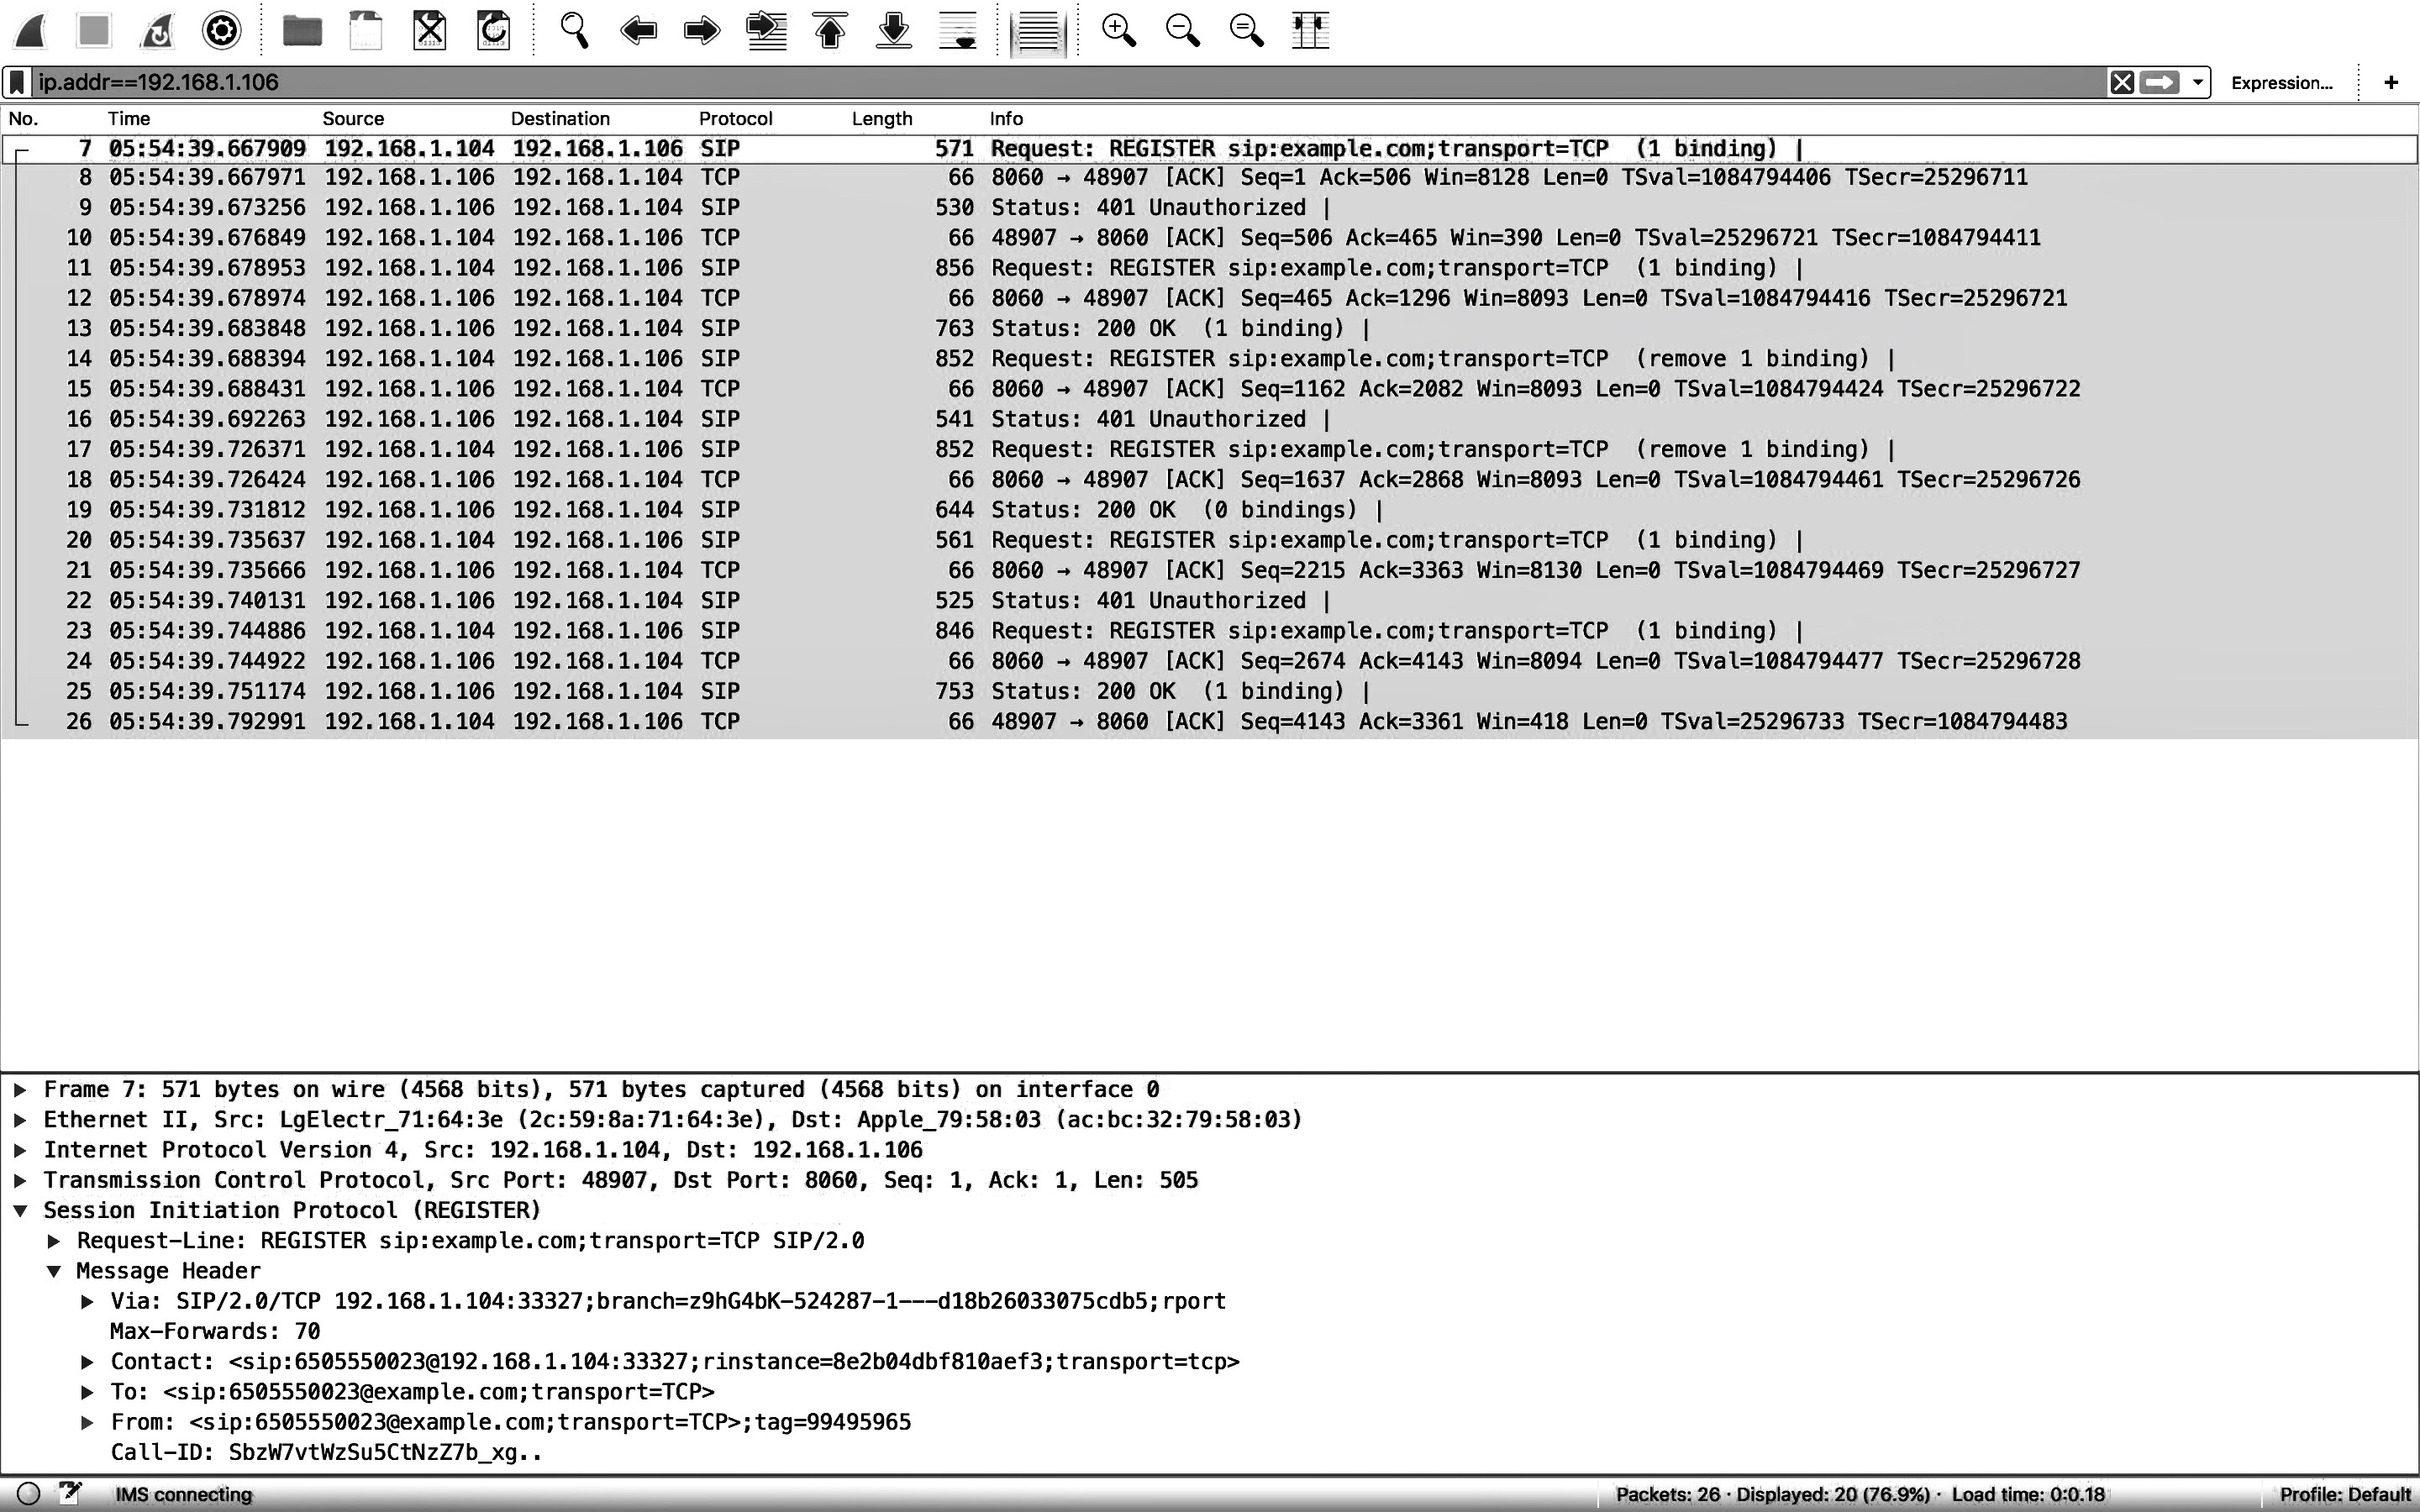
\includegraphics[width=\textwidth]{imssip}
\caption{پیام\nf های مبادله\nf شده برای ثبت\nf نام \lr{SIP} در \lr{IMS}}
\label{imssip}
\end{figure}

\begin{figure}[h]
\centering
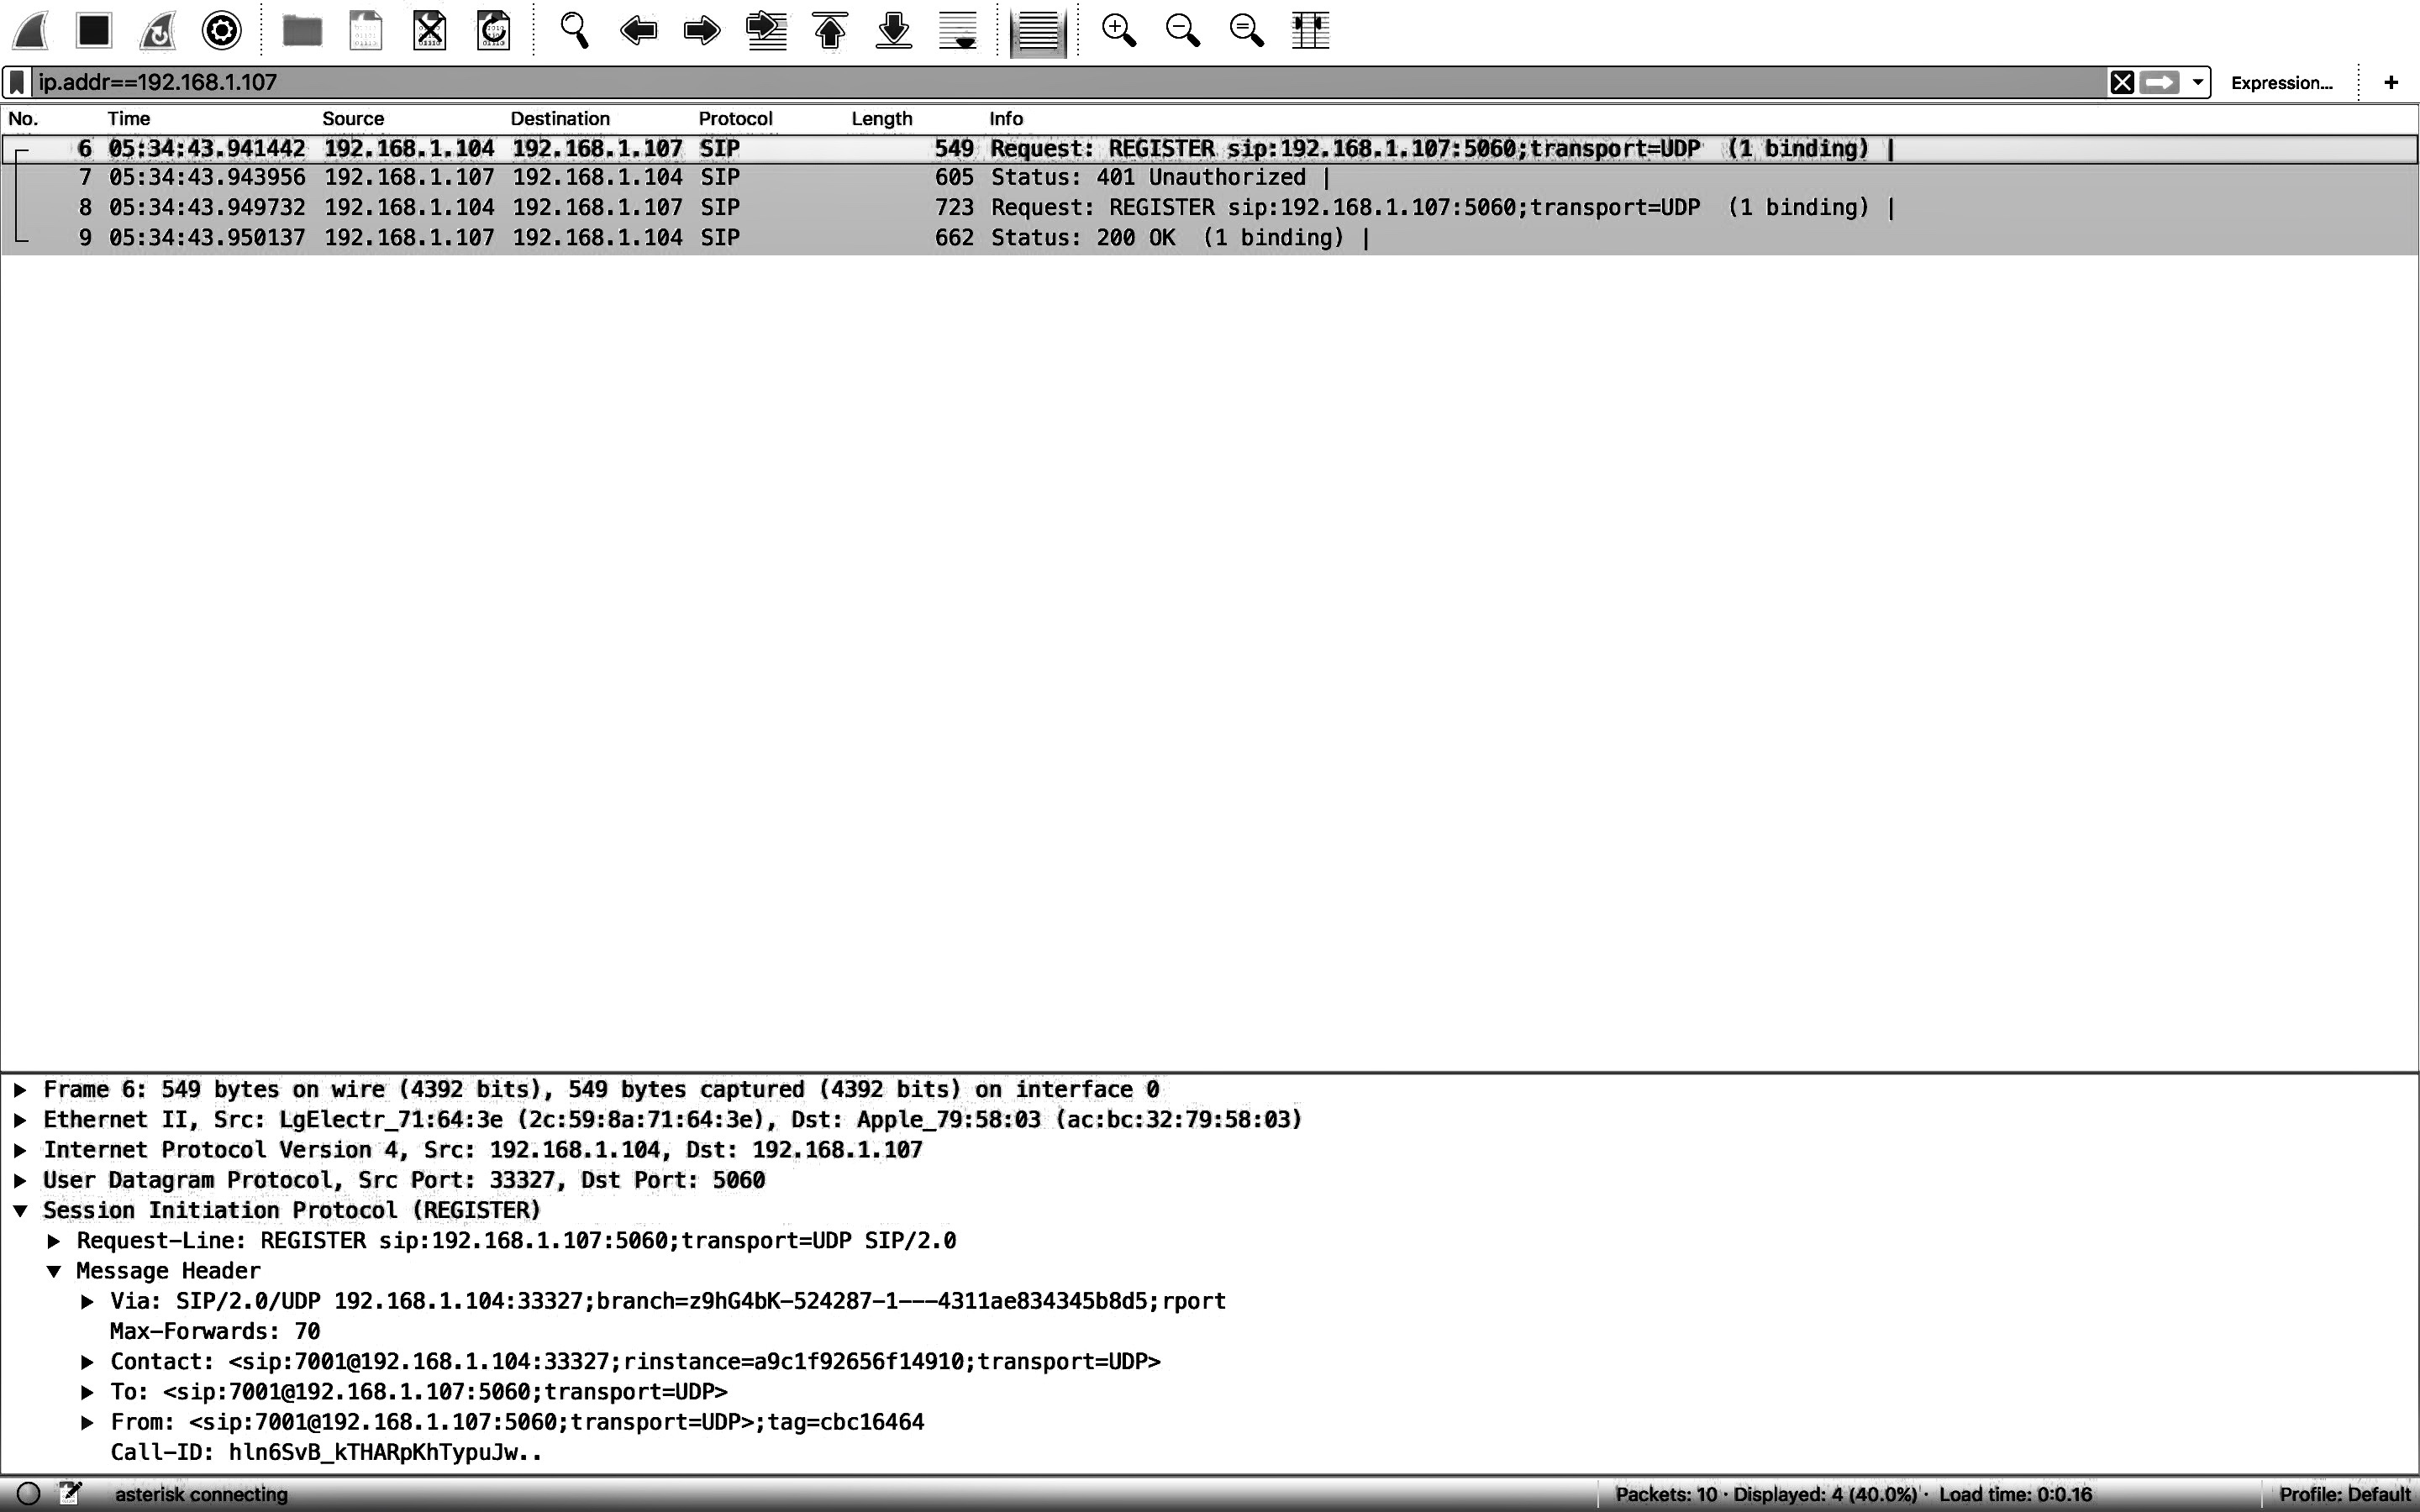
\includegraphics[width=\textwidth]{voipsip}
\caption{پیام\nf های مبادله\nf شده برای ثبت\nf نام \lr{SIP} در \lr{VOIP}}
\label{voipsip}
\end{figure}

مطابق مطالب گفته\nf شده در بخش \ref{archPart}، المان \lr{I-CSCF} باید در هنگام ثبت\nf نام، نود \lr{S-CSCF}  مناسب را به دستگاه کاربر اختصاص دهد. در آخرین مرحله از ثبت\nf نام \lr{SIP} در \lr{IMS}، نود \lr{S-CSCF} اختصاص\nf یافته به کاربر به\nf همراه شماره پورت مورد استفاده و همچنین آدرس \lr{IP} ماشین مجازی \lr{clearwater} که در پشت \lr{NAT} قرار دارد، برای کاربر ارسال می\nf شود. این اطّلاعات، در شکل \ref{imssiproute} مشخّص شده\nf اند.

همچنین، سیگنالینگ\nf های استفاده\nf شده در \lr{IMS} و \lr{VOIP} برای ایجاد جلسه و برقرای تماس تلفنی نیز به همین روش مورد بررسی قرار گرفت. با وجود تفاوت\nf های جزئی در پیام\nf های مبادله\nf شده، هر دو سیستم از استانداردهای پروتکل \lr{SIP} پیروی می\nf کنند. مدّت\nf زمانِ ایجاد جلسه در هر دو سیستم، تقریباً یکسان است و نتایجی مشابه نتایج مقایسه\nf ی سیگنالینگ\nf های ثبت\nf نام \lr{SIP} به\nf دست آمد. لذا از ارائه\nf ی جزئیات مربوط به این مقایسه، اجتناب شده است.

\begin{figure}[H]
\centering
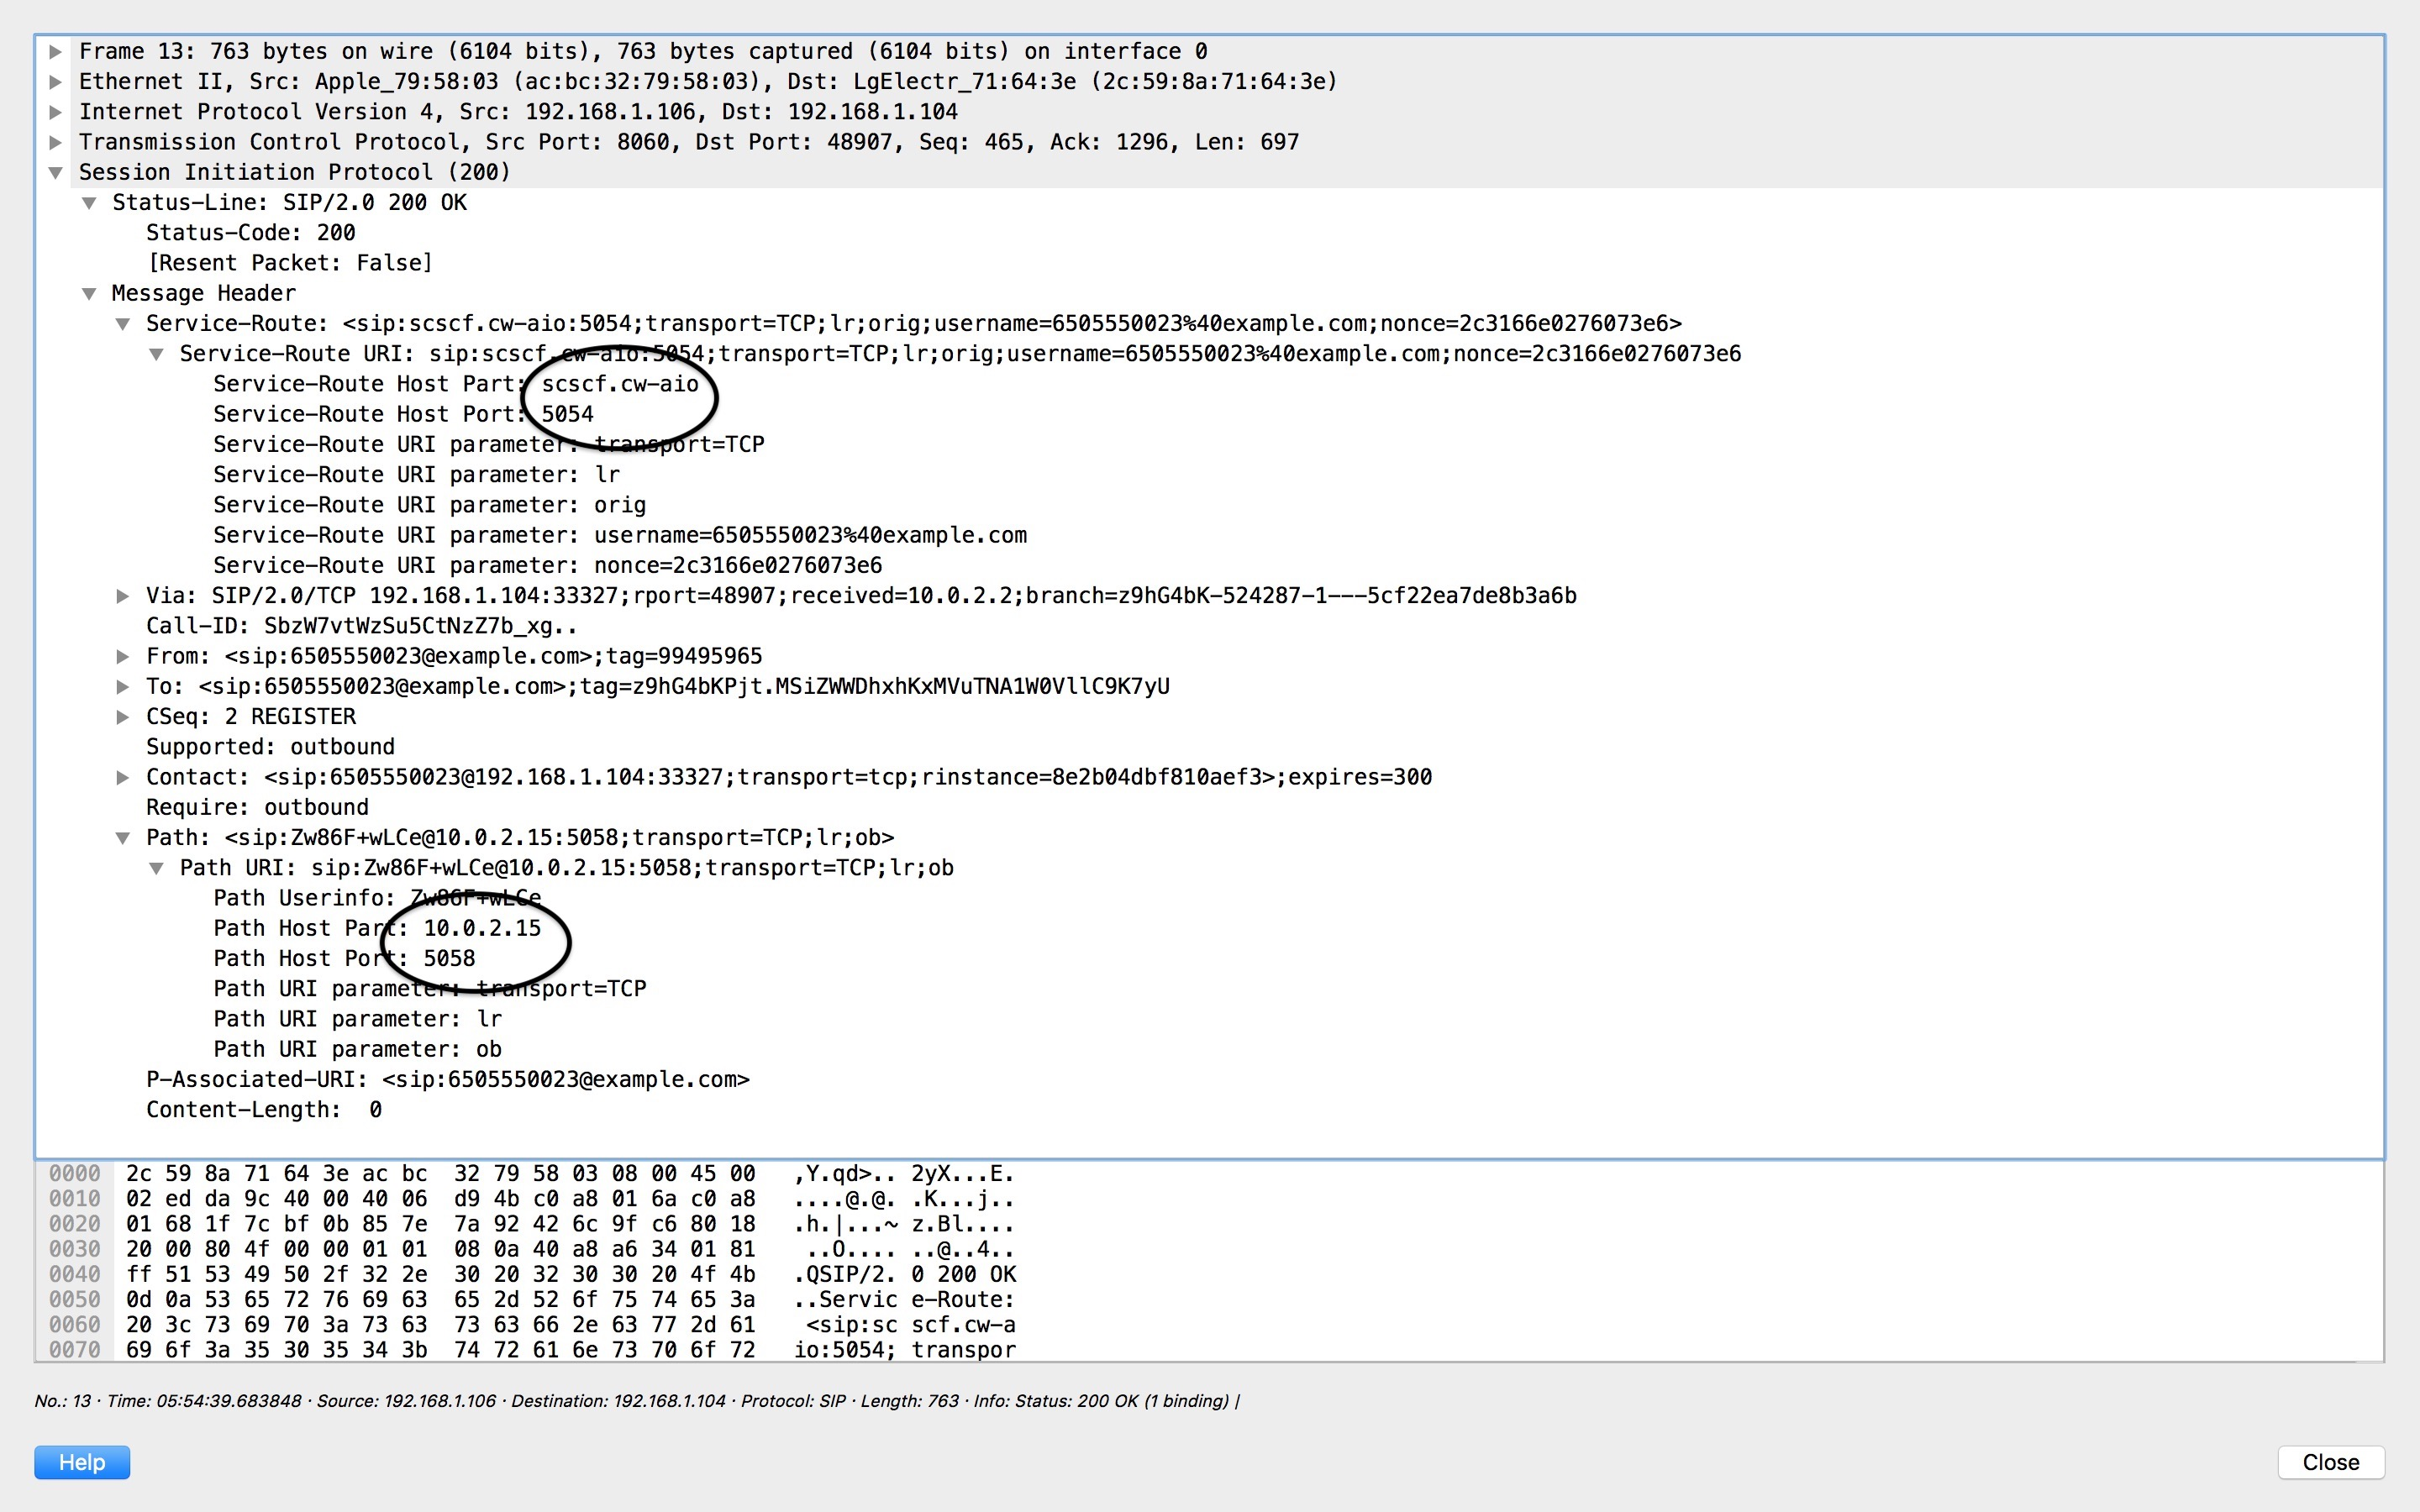
\includegraphics[width=\textwidth]{imssiproute}
\caption{اطّلاعات ارسال\nf شده به کاربر در آخرین مرحله\nf ی ثبت\nf نام \lr{SIP} توسّط سرور \lr{IMS}}
\label{imssiproute}
\end{figure}

 

\section{مقایسه\nf ی کیفیّت سرویس در شبکه سلولی}

برتری اصلی \lr{IMS} نسبت به سیستم\nf های \lr{VOIP} کنونی،فراهم کردن کیفیت سرویس است. امّا همانطور که در بخش\nf های قبل گفته\nf شد، در صورت استفاده از \lr{IMS} به\nf عنوان سرور \lr{VOIP}، چینین مزیّتی وجود ندارد. برقراری کیفیّت سرویس توسّط \lr{IMS}، مربوط به کنترل بستر مدیای شبکه\nf ی سلولی و کنترل بخش شبکه\nf ی دسترسی رادیویی است. \lr{IMS} می\nf تواند از طریق ارتباط با المان\nf های شبکه\nf ی سلولی در ناحیه\nf ی دسترسی رادیویی و همچنین المان\nf هایی که بستر عبور مدیا در شبکه\nf ی سلولی را فراهم می\nf کنند، کیفیت سرویس موردنیاز کاربران را فراهم کند. سیستم\nf های \lr{VOIP} متداول، چنین قابلیتی را ندارند.

کیفیت سرویسی که \lr{IMS} برای هر جلسه فراهم می\nf کند، به عوامل مختلفی بستگی دارد. عامل اوّل، پروفایل کاربر موردنظر می\nf باشد. کاربرانی که سرویس طلایی را خریداری می\nf کنند، نسبت به کاربران عادّی کیفیت سرویس بهتری را دریافت می\nf کنند. عامل دیگر، نوع سرویس مورد استفاده است. استاندارد \lr{3gpp}، چهار کلاس کیفیت سرویس را تعریف کرده است که به آن، کلاس ترافیک نیز می\nf گویند. کلاس\nf های ترافیک، به ترتیب اولویّت برای دریافت کیفیت سرویس بالاتر، به شرح زیر هستند\cite{blended}
\begin{enumerate}
\item کلاس مکالمه: مانند مکالمات صوتی و ویدیوئی
\item کلاس \lr{streaming}: مانند تماشای ویدیوهای زنده و یا از قبل ضبط\nf شده به صورت آنلاین
\item کلاس تعاملی\RTLfootnote{\lr{Interactive}}:مانند وب\nf گردی
\item کلاس پس\nf زمینه\RTLfootnote{\lr{Background}}: مانند پست الکترونیک
\end{enumerate}

المان \lr{PCRF} در معماری \lr{IMS}، مسئول برقراری ارتباط با المان\nf های معماری شبکه\nf ی سلولی و فراهم کردن کیفیت سرویس است. این المان، معمولاً به\nf عنوان بخشی از المان \lr{P-CSCF} پیاده\nf سازی می\nf شود\cite{blended}. در پیاده\nf سازی \lr{clearwater}، المان \lr{Bono} نقش \lr{P-CSCF} را دارد. المان \lr{Bono} که به\nf صورت متن\nf باز پیاده\nf سازی شده است، فاقد المان \lr{PCRF} بوده و کیفیت سرویس را فراهم نمی\nf کند. شرکت \lr{Metaswitch} که پروژه\nf ی \lr{clearwater} را راه\nf اندازی کرده و رهبری می\nf کند، المانی به نام \lr{Perimeta} را به\nf عنوان محصولی تجاری، ارائه می\nf کند. این المان که یک کنترل\nf کننده\nf ی مرز جلسه است، به\nf جای المان \lr{Bono} در معماری \lr{clearwater} قرار می\nf گیرد. با استفاده از \lr{Perimeta}، ارتباط \lr{clearwater} با شبکه\nf ی سلولی برقرار می\nf شود. \lr{Perimeta}، علاوه بر فراهم کردن کیفیت سرویس، خدمات شارژینگ را نیز انجام می\nf دهد\cite{webperimeta}. به\nf دلیل در اختیار نداشتن این محصول تجاری(و گران\nf قیمت بودن آن)، امکان بررسی کیفیت سرویسِ فراهم\nf شده توسّط \lr{IMS} در شبکه\nf ی سلولی، وجود ندارد؛ امّا با توجّه به ادّعای شرکت \lr{Metaswitch} و نظرات مشتریانی که از \lr{Perimeta} استفاده کرده\nf اند، می\nf توان قبول کرد که پیاده\nf سازی \lr{claerwater}، توانایی فراهم کردن کیفیت سرویس در شبکه\nf ی سلولی را دارد.


